% ----------------------------------------------------------
% Teste test2_1_e5b64class10_20231211_220210
% ----------------------------------------------------------
\subsubsection{Teste test2_1_e5b64class10_20231211_220210 - AlexNet (Is That a Santa)}

Informações utilizadas para o treinamento.

\begin{table}[ht]
   \centering
   \caption{Treinamento}
   \label{tab:modelos}
   \begin{tabular}{| c | c | }
      \hline 
      \textbf{Informação} & \textbf{Descrição} \\
      \hline \hline 
      Rede & AlexNet \\
      \hline
      Número de épocas & 5\\
      \hline
      Tamanho do lote & 64\\
      \hline
      Taxa inicial & 0.01 \\
      \hline
      Taxa de decaimento & 0.0005 \\
      \hline
      Total de classes & 10\\
      \hline
      Dataset & CIFAR-10\\
      \hline
   \end{tabular} 
\end{table}

Resultados obtidos após treinamento.

\begin{tabular}{lrrrr}
\toprule
  Unnamed: 0 &  precision &  recall &  f1-score &    support \\
\midrule
    airplane &   0.750868 &  0.8650 &  0.803903 &  1000.0000 \\
  automobile &   0.800681 &  0.9400 &  0.864765 &  1000.0000 \\
        bird &   0.688119 &  0.6950 &  0.691542 &  1000.0000 \\
         cat &   0.609707 &  0.6030 &  0.606335 &  1000.0000 \\
        deer &   0.642857 &  0.8550 &  0.733906 &  1000.0000 \\
         dog &   0.778319 &  0.6390 &  0.701812 &  1000.0000 \\
        frog &   0.862288 &  0.8140 &  0.837449 &  1000.0000 \\
       horse &   0.901515 &  0.7140 &  0.796875 &  1000.0000 \\
        ship &   0.867925 &  0.8740 &  0.870952 &  1000.0000 \\
       truck &   0.919334 &  0.7180 &  0.806289 &  1000.0000 \\
    accuracy &   0.771700 &  0.7717 &  0.771700 &     0.7717 \\
   macro avg &   0.782161 &  0.7717 &  0.771383 & 10000.0000 \\
weighted avg &   0.782161 &  0.7717 &  0.771383 & 10000.0000 \\
\bottomrule
\end{tabular}


\begin{figure}[ht]
 \begin{center}
   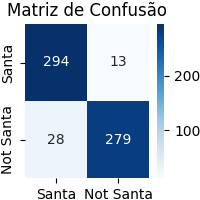
\includegraphics[scale=1]{tests/test2_1_e5b64class10_20231211_220210/confusion_matrix.png}
  \caption{Matriz de Confusão}
  \label{fig:fig03}
 \end{center}
\end{figure}

\begin{figure}[ht]
 \begin{center}
   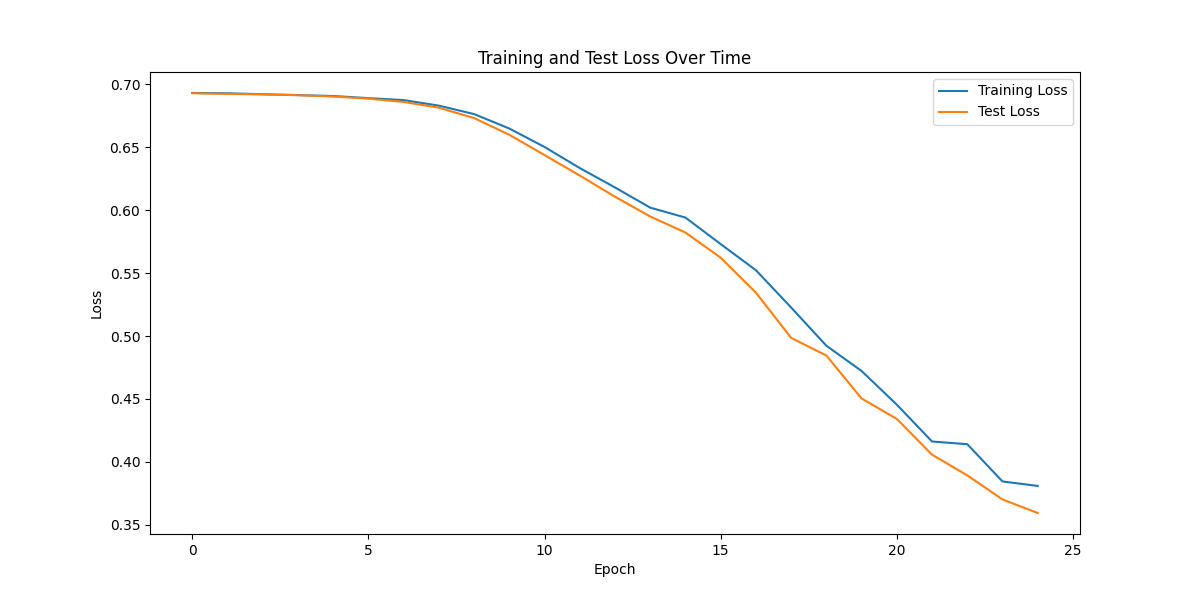
\includegraphics[scale=0.8]{tests/test2_1_e5b64class10_20231211_220210/loss_over_time.png}
  \caption{Gráfico de Perda}
  \label{fig:fig04}
 \end{center}
\end{figure}
